%!TEX root = ../thesis.tex
\glsresetall

\chapter{Introduction}
\label{chap:intro}

\Gls{it} is constantly shaping the world that we live in. Its advancements have changed human behavior and influenced the way we connect with our environment. Music being a universal socio-cultural phenomena has been deeply influenced by these advancements. The way music is created, stored, disseminated, listened to, and even learned has changed drastically over the last few decades. A massive amount of audio music content is now available on demand. Thus, it becomes necessary to develop computational techniques that can process and automatically describe large volumes of digital music content to facilitate novel ways of interaction with it. There are different information sources such as editorial metadata, social data, and audio recordings that can be exploited to generate a description of music. Melody, along with harmony and rhythm, is a fundamental facet of music, and therefore, an essential component in its description. In this thesis, we focus on describing melodic aspects of music through an automated analysis of audio content. 

\section{Motivation}
\label{sec:motivation}

\blockcquote[]{selfridge1998conceptual}{``\textit{It is melody that enables us to distinguish one work from another. It is melody that human beings are innately able to reproduce by singing, humming, and whistling. It is melody that makes music memorable: we are likely to recall a tune long after we have forgotten its text.}''}

The importance of melody in our musical experiences makes its analysis and description a crucial component in music content processing. It becomes even more important for melody dominant music traditions such as \gls{iam}, where the concept of harmony (functional harmony as understood in common practice) does not exist, and the complex melodic structure takes the central role in music aesthetics.

Melodic analysis and description is not a recent phenomenon, it has been done by musicologists for hundreds of years. However, a computational approach to this task has opened up new directions and possibilities, taking it to a different scale altogether. Through computational approaches, melodic analysis and description can be performed at the level of an entire music repertoire, as opposed to a few music pieces typically considered in manually performed musicological studies. Needless to say that such computational analysis is work in progress with continuous attempts to improve the quality of the outcomes, so that they closely resemble to what can be done by human experts.

Most of the current computational approaches that analyze high-level melodic aspects of music such as melodic similarity and motifs work with its symbolic representations, thus covering only a particular view of music. There are significant challenges in extending such approaches to analyze recorded performances, mainly due to the difficulties involved in obtaining a meaningful symbolic representation from audio recordings. Therefore, for performance oriented music traditions such as \gls{iam}, where symbolic music representations are practically nonexistent and the aesthetics lie in the improvisatory aspects, such approaches are not directly applicable. Besides, melody, being a cultural phenomenon, should be studied within the cultural context of a music tradition. Thus, there is a need to develop culture-aware computational approaches that exploit the specificities of a music tradition to analyze and describe the melodic aspects of recorded music performances. \gls{iam} with its complex melodic framework, \gls{raga}, and well grounded-music theory, provides an ideal context to develop such approaches.

Melodic elements in \gls{iam} are hierarchically organized in accordance with the \gls{raga} grammar. At the lowest level there are \glspl{svara}, which concatenate to form melodic phrases. These phrases group together to form passages, finally leading to a music piece. At each level these melodic elements adhere to the \gls{raga} grammar. In this thesis we focus on computational approaches that analyze these melodic elements at different hierarchical levels to describe melodic aspects of \gls{iam} corpora. 

Automated analysis and description of high-level melodic aspects of \gls{iam} has manifold applications. It can enable corpora level musicological studies such as characterization of music compositions, artists and \glspl{raga}. Since \gls{iam} follows an oral pedagogy, analysis of the recorded performances can shed light on the stylistic influences of teachers on their students, and to other artists. Establishing relationships between different melodic elements across recordings in a music collection opens up ways to define novel music similarity measures, and generate semantically meaningful description in terms of higher level melodic concepts, such as \glspl{raga}. This further enables several applications such as structuring and organizing large music archives, \gls{raga}-based music retrieval and culturally relevant music navigation and discovery. A rich description of different melodic elements can aid immensely in developing novel applications that address enhanced or augmented music listening experience. This aspect is specifically relevant in the case of \gls{iam}, wherein the music is largely accessible (in terms of the understanding) to musicians and music connoisseurs owing to the complexity of the melodic structures. Furthermore, being able to analyze and characterize different melodic elements directly from the audio recordings opens up novel and creative ways to approach music pedagogy. Specifically in the context of \gls{iam}, where the music nuances are learned implicitly through years of training, an objective description of melodic aspects can aid music students to learn from the recorded performances of maestros. 


\section{Scientific Context}
\label{sec:context}

\Gls{mir} is a growing interdisciplinary research field that stands at the intersection of well established disciplines such as signal processing, pattern recognition, musicology, psychoacoustics, music perception and cognition, information science, and computer science. \Gls{mir} primarily addresses topics involved in the understanding and modeling of music using information processing methodologies~\citep{roadmap_mir}. In particular, it aims to advance our knowledge in representing, understanding, describing, retrieving, archiving and organizing music related data. This opens up a wealth of possibilities to develop novel ways to interact with music~\citep{casey2008content,orio2006music,burgoyne2016music}. 

The field of \gls{mir} has made significant progress in the last two decades. Its growth is fueled by the massive surge in the digital music content. A large number of \gls{mir} systems aim to describe and characterize music content in terms of different musical facets such as melody, rhythm, harmony, structure and emotion. The definition, interpretation and relevance of these musical aspects are not universal and vary significantly across different music traditions and personal, cultural, and social contexts. A significant number of existing computational approaches in \gls{mir} fail to account for these factors, and thus, might be hitting the so-called ``glass ceiling"~\citep{pachet2004improving,casey2008content}. In addition, there also exists a semantic-gap between the automatically extracted music descriptors from audio signals and the high-level music concepts that humans relate to~\citep{celma2006foafing,casey2008content}. Furthermore, since the research problems undertaken in \gls{mir} have mainly been shaped by the western commercial music of the past few decades, many of the technologies developed within \gls{mir} are not directly applicable to several other music traditions of the world~\citep{XavierSerra2011}. Thus, there is a need to bridge this gap and take a broader perspective to describe music by taking the cultural, social and the user context into account~\citep{roadmap_mir}. It is in this context that the CompMusic project was envisioned.

CompMusic\footnote{http://compmusic.upf.edu/} (Computational Models for the Discovery of the World's Music) is a research project funded by the European Research Council~\citep{XavierSerra2011}. The project focuses on five music traditions of the world: Hindustani (North India), Carnatic (South India), Turkish-makam (Turkey), Arab-Andalusian (Maghreb), and Beijing Opera (China). One of the main objectives of the CompMusic project is to promote and develop multicultural perspectives in \gls{mir}. In particular, the project aims to advance the research in computational description of music by identifying musically relevant problems coming from culture-specific contexts and developing domain specific approaches to solve them. Addressing the research problems in the context of diverse music cultures will not only help in advancing the knowledge in the specific cultures, but also expand the scope of the current research in \gls{mir}. It can also help bridge the semantic gap and push the glass ceiling. 

CompMusic project follows a data-driven research methodology. The efficacy of the computational approaches following such methodologies are directly impacted by the quality of the data using which they are developed. Thus, one of the goals in the CompMusic project is to create quality data corpora that are representative of the performance practices of the music traditions. The corpora compiled and curated in the CompMusic project mainly comprise commercial quality audio recordings and relevant editorial metadata. 

The work presented in this dissertation is carried out as a part of the CompMusic project and aligns with its goals. In this thesis, we focus on analysis and description of melodic aspects in \gls{iam} corpora. Our efforts are directed towards the bigger goal of developing culture-aware computational approaches that can utilize domain knowledge in order to produce semantically meaningful description of music. The cultural specificities of \gls{iam} have shaped our work at each step, whether it is the identification of relevant research problems, building the data corpora, or the methodology adopted by the computational approaches. The insights gained in the process of developing culture-aware and domain specific approaches will help expand the scope of the state of the art in \gls{mir}. Our work also paves way for cross-cultural studies, which can help us better understand the influence of the cultural training on perception and cognition of different musical aspects.



\section{Opportunities and Challenges}
\label{sec:challenges_opportunities}

\gls{iam} is a highly evolved music tradition with its origins dating back as early as 1500\,BC, and is alive and thriving. It is a well studied music tradition with sophisticated and grounded music theory. The literature is replete with scholarly text written on musical concepts in \gls{iam}. However, this music tradition is not explored fully from a computational analysis point of view. The established music theories and existing musicological work provides a strong base to formulate \gls{mir} tasks and develop computational models for automatic music description.

\gls{iam} is a performance centric music tradition, which has been transmitted orally across generations following a tradition of Guru-Shishya parampara (``lineage'' system). The musical compositions in \gls{iam} merely act as skeletons in music performances, and the essence of the music lies in the improvisatory aspects. As a result of which, \gls{iam} mainly possesses recorded music repertoire. 

Reliable extraction of even a low-level melody representation such as predominant pitch from recorded performances is a challenging task. As a result of which, computational approaches for melodic description in audio recordings are still primarily focused on extracting such representations and have not been able to address higher level melodic analyses comprehensively. Specific heterophonic characteristics of \gls{iam} make it feasible to obtain a low-level melody representation from audio recordings using the current state of the art predominant pitch estimation methods. This is also indicated by the past MIREX (an international \gls{mir} evaluation campaign) results\footnote{\url{http://www.music-ir.org/mirex/wiki/MIREX_HOME}}. Compare the accuracy obtained by different algorithms on INDIAN08\footnote{\url{http://nema.lis.illinois.edu/nema_out/mirex2011/results/ame/indian08/summary.html}}, MIREX05\footnote{\url{http://nema.lis.illinois.edu/nema_out/mirex2011/results/ame/mirex05/summary.html}} and MIREX09~0dB\footnote{\url{http://nema.lis.illinois.edu/nema_out/mirex2011/results/ame/mirex09_0dB/summary.html}} datasets from MIREX-2011. The feasibility of obtaining a reasonably accurate predominant pitch representation of melody from audio recordings enables us to focus on the description of higher level melodic aspects of music performances. Thus, \gls{iam} provides an opportunity to broaden the scope of computational approaches for melodic analysis and description much beyond describing the melodic aspects of music performances by merely the pitch contours.

Although the extraction of predominant pitch in \gls{iam} recordings is relatively less complicated, its abstraction into a symbolic representation is a challenging task. One way of abstracting a continuous pitch contour is by performing melody transcription, which is still a challenging and an ill-defined task in the case of \gls{iam}, primarily due to its meandering melodic characteristics~\citep{widdess1994involving,rao1999raga}. Moreover, the process of discretization of such melodic movements may result in a loss of information relevant to the characterization and description of melodies. Thus, difficulties in abstraction of a continuous melody representation in \gls{iam} poses challenges in its processing. 

There is no standard frequency that is used as a reference for tuning instruments and voice in the performances of \gls{iam}. A lead artist can choose any convenient frequency as tonic, which acts as the reference using which all accompanying instruments are tuned. Tonic pitch varies across artists and may also vary across the performances of an artist. These factors make it difficult to directly process melodies across different artists as well as across different performances of an artist.

\blockcquote[]{Cambouropoulos2006}{``\textit{Music becomes intelligible to a great extent through self-reference, i.e., through the relations of new musical passages to previously heard material. Structural repetition and similarity are crucial devices in establishing such relations.''}}

\blockcquote[]{schenker1980harmony}{``\textit{Only by repetition can a series of tones be characterized as something definite. Only repetition can demarcate a series of tones and its purpose. Repetition thus is the basis of music as an art.}''}

Analysis of repeating melodic patterns has been instrumental in the description of melodies, and is therefore utilized by a large number of computational approaches in \gls{mir}. Repeating melodic patterns are integral to the melodic framework in \gls{iam}, the \gls{raga}. They act as building blocks to construct melodies within the \gls{raga} grammar. There are different types of melodic patterns in \gls{iam} with their well defined functional roles. For example, a certain type of patterns correspond to melodic ornaments, some others form the opening line of compositions and, musically the most significant patterns are those that characterize \glspl{raga} (\secref{sec:music_background}). Thus, \gls{iam} provides an interesting opportunity to develop computational approaches for discovery and characterization of melodic patterns from audio collections. However, the improvisatory nature of this music tradition makes this task challenging. The characteristic melodic phrases of \glspl{raga} act as the basis for artists to improvise, providing them with a medium to express creativity during \gls{raga} rendition. Artists bring in novelty through creatively transforming these melodic phrases as much as possible within the periphery defined by the \gls{raga} grammar. Therefore, the surface representation of these melodic phrases vary a lot across their occurrences. This high degree of variation in terms of the overall duration of a phrase, non-linear time warpings and the added melodic ornaments together pose a big challenge for melodic similarity computation and pattern extraction in \gls{iam}. In~\figref{fig:phraseComplexityExample_intro} we illustrate this variability by showing the pitch contours of the different occurrences of three characteristic melodic phrases of \gls{raga} \gls{alahaiya_bilaval}. We can clearly see that the duration of a phrase across its occurrences varies a lot, and the steady melodic regions are highly varied in terms of the duration and the presence of melodic ornaments. These characteristics of the melodic patterns in \gls{iam} provide an opportunity to gain deeper insights into the perception of melodic similarity as well as how it is influenced by the cultural aspects. 

\begin{figure}
	\begin{center}
		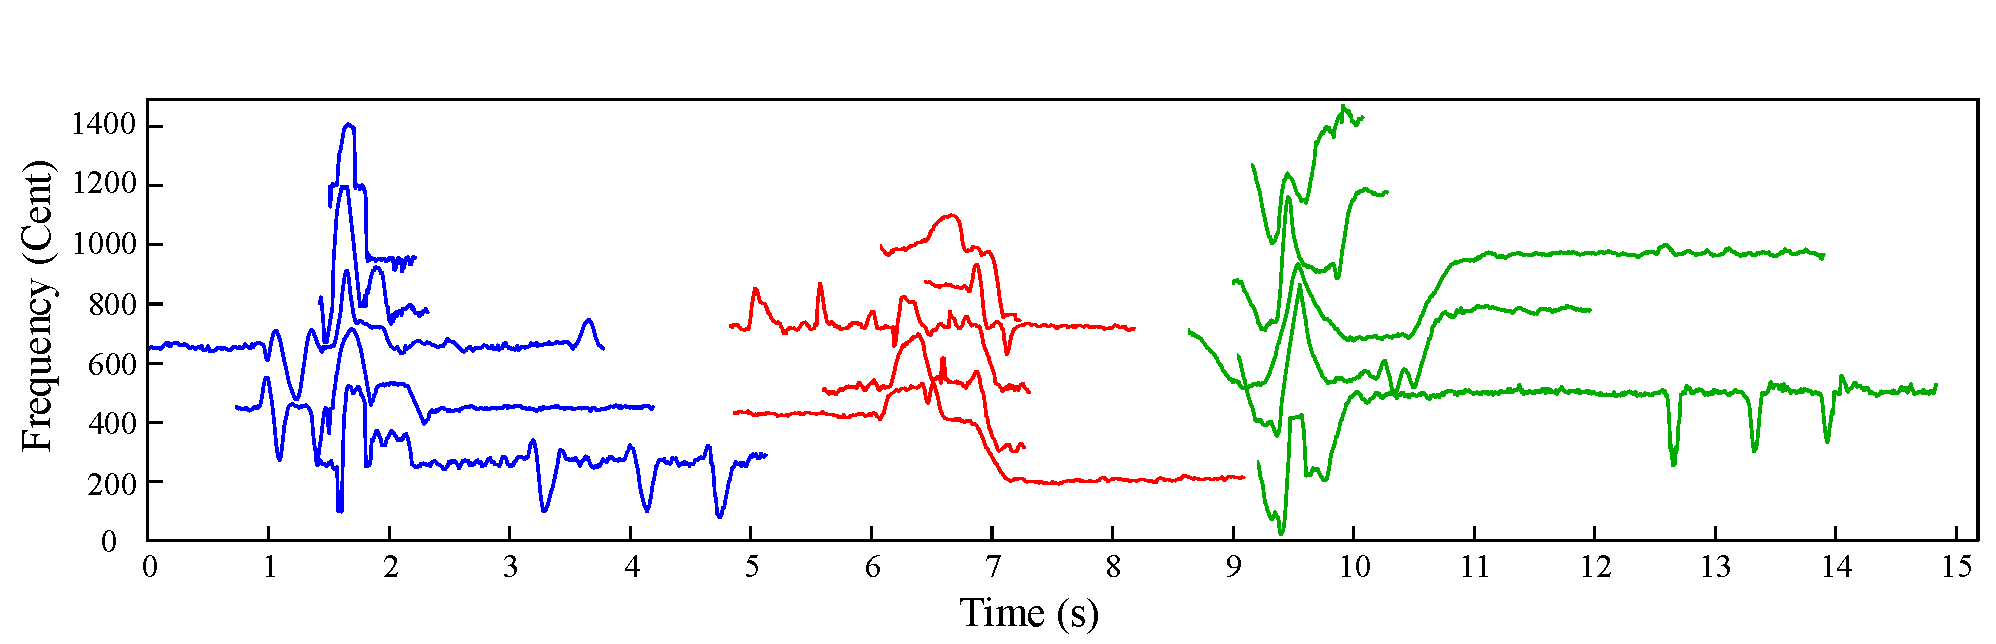
\includegraphics[width=\figSizeHundred]{ch01_introduction/figures/phraseClassesExample.pdf}
	\end{center}
	\caption[Examples of the characteristic melodic phrases in Hindustani Music]{Pitch contours of occurrences of three different characteristic melodic phrases in Hindustani music. Contours are frequency transposed and time shifted for a better visualization.}
	\label{fig:phraseComplexityExample_intro}
\end{figure}

Discovery of melodic patterns is a computationally complex task, specifically when performed using music parallelism~\citep{Cambouropoulos2006}. It becomes even more challenging in the case of \gls{iam} given the long duration of the audio recordings, some of which may even last for an hour.

\blockcquote[p. 96]{martinez2001semiosis}{``\textit{The \gls{raga} is more fixed than a mode, and less fixed than the melody, beyond the mode and short of melody, and richer both than a given mode or a given melody.}''}


\blockcquote[]{powers1963background}{``\textit{A \gls{raga} is not a tune, nor is it a `modal' scale, but rather a continuum with scale and tune as its extremes.}''}

\Gls{raga} thus is a fascinating topic of research, specifically in the context of \gls{mir}. Being a complex melodic framework it involves an intricate interplay between different melodic elements both in terms of the tonality and their temporal relations. Therefore, its computational characterization and recognition poses unique challenges as well as provides new opportunities. It is worth mentioning that recognizing \gls{raga} in a musical performance requires domain expertise, which further emphasizes the complexity of the task.

\gls{iam} thus provides a context that is highly conducive to developing novel computational approaches to describe higher level melodic aspects of music, specifically in collections of recorded performances. 


\section{Scope and Objectives}
\label{sec:scope_objectives}

Analysis and description of melodic aspects of music is a broad research topic that can be approached from a number of perspectives and different academic disciplines. In this thesis we take a data-driven engineering approach and focus solely on the computational aspects of melodic analysis, making use of established music theories. Our applied research methodology stands at the intersection of signal processing, machine learning and time-series analysis. We focus on content-based processing, wherein the input data to our approaches comprise mainly audio recordings, and in a few cases their associated editorial metadata. The approaches proposed in our work are developed and evaluated using music collections of \gls{iam} that includes both Hindustani and Carnatic music. We now outline our broad objectives in this thesis.

\begin{itemize}
	\item To curate and structure representative music corpora of \gls{iam} that comprise audio recordings and associated metadata, and use that to compile sizable and well annotated tests datasets for melodic analyses.
	\item To develop data-driven computational approaches for discovery and characterization of musically relevant melodic patterns in sizable audio collections of \gls{iam}
	\item To devise computational approaches for automatically recognizing \glspl{raga} in recorded performances of \gls{iam}.
\end{itemize}

In order to achieve these broad objectives, there are a number of computational tasks pertaining to melodic analysis of \gls{iam} that are addressed in this thesis. A visual summary of these tasks is provided in~\figref{fig:tasks}. We now briefly enumerate these tasks.

Melodies in \gls{iam} need to be analyzed within their tonal context set by the tonic pitch of the lead performer. Therefore, automatic tonic identification becomes the first step in melodic analysis of this music. Though a number of methods are proposed for this task, including our own, there is no consensus on the best performing approach as they are evaluated on different datasets and experimental conditions~\citep{Gulati2014Tonic}. In this thesis we aim to perform an exhaustive comparative evaluation of different tonic identification approaches on a variety of music material to select the most robust and accurate approach to be used in our work. 

An important step in analyzing melodies, specifically in a pattern-based analysis, is the identification of meaningful melodic segments. We aim to devise a segmentation approach that can facilitate melodic pattern processing tasks in \gls{iam}. 

Computation of melodic similarity is critical in pattern processing of melodic sequences. Since characteristics of melodies in \gls{iam} differ significantly from those in several other music traditions, it becomes important to investigate thoroughly the influence of different melody representations, melody normalization strategies and similarity measures on the computation of melodic similarity for this tradition. Such an analysis will not only reveal the challenges involved in the task, but will also help in identifying ways in which specific peculiarities of this music tradition can be exploited for improving melodic similarity. 

Discovery of short-duration melodic patterns in audio recordings is a challenging task. It becomes even more challenging when the discovery is performed at the level of an entire corpus that spans hundreds of hours of audio content. We aim to develop a methodology to mine meaningful repeating melodic patterns in large audio collections of \gls{iam}. 

The characteristics and the functional roles of repeating melodic patterns vary a lot across music traditions. For some music traditions frequently occurring patterns might be the most important ones. Whereas, in some others, highly repetitive patterns might be musically trivial. Characterization of the melodic patterns should thus be studied within the context of a specific music tradition. We aim to develop an approach that can exploit domain-specific knowledge to effectively characterize melodic patterns in \gls{iam}.

\begin{figure}
	\begin{center}
		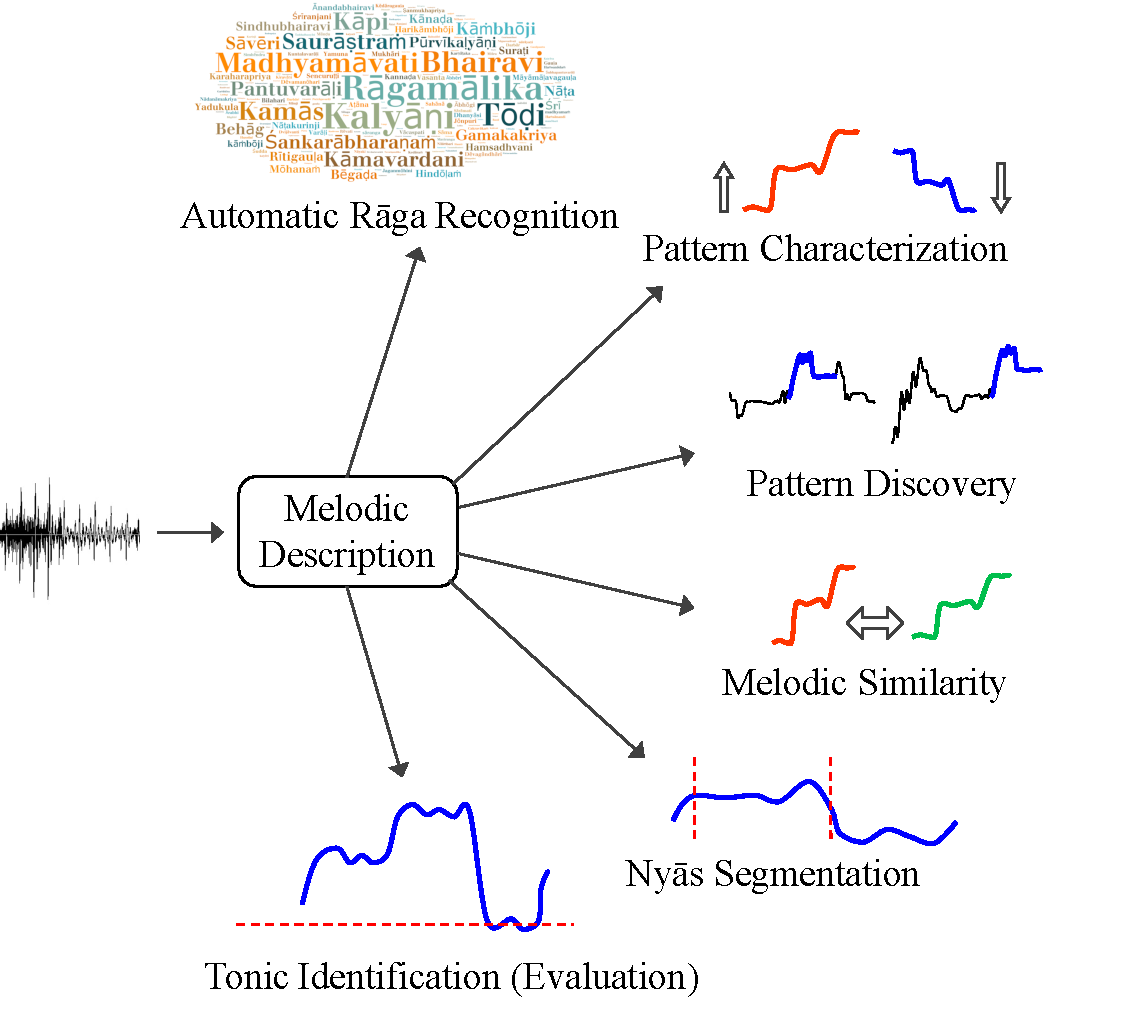
\includegraphics[width=\figSizeSeventyFive]{ch01_introduction/figures/tasks.pdf}
	\end{center}
	\caption[Computational melodic analyses addressed in this thesis]{Computational tasks within melodic analysis of \gls{iam} that are addressed in this thesis.}
	\label{fig:tasks}
\end{figure}

Finally, we aim to investigate one of the most studied and relevant topics in computational analysis of \gls{iam}, automatic \gls{raga} recognition. Our goal is to devise an approach that can successfully utilize both the tonal and the temporal characteristics of melody to perform the task. 

Our work aligns with the philosophy of open-access and reproducible research. The data and the code pertaining to this thesis is made publicly available online (\appref{app:resources}). 

\section{Thesis Outline}
\label{sec:intro_thesis_outline}

There are eight chapters in this thesis, wherein the primary contributions are contained in Chapter 3 to 6. Each of these chapters contains an introduction, the main body and a summary of the key results and conclusions. A significant amount of the content in these chapters is derived from our publications~\cite{Gulati2014Tonic,gulati2014Landmark,gulati_SITIS_2014,gulati_ICASSP2015,gulati_ISMIR_2015,gulati_communities_2016,gulatiphrase_2016,gulati_tdms_2016}. Most of the work in these papers is done in collaboration with other researchers and musicians, which is duly indicated wherever required. 

In \chapref{chap:background}, we provide an overview of the music and scientific background, with emphasis on the existing literature relevant to the work presented in this thesis. We start with a brief introduction to \gls{iam} and its music concepts pertaining to melody (\secref{sec:music_background}). We present our review of current computational approaches for tonic identification, \gls{raga} recognition and melodic pattern processing in the context of \gls{iam} (\secref{sec:background_relevant_work_iam}). We critically analyze and compare these approaches in terms of algorithmic design and evaluation methodology, in which we highlight their shortcomings and identify potential avenues of scientific contributions. In addition, we also present a brief review of the existing literature on tonality modeling and pattern processing in \gls{mir}, covering topics such as structural segmentation, motivic analysis and \gls{qbh} (\secref{sec:background_relevant_work_other_music}).

In \chapref{chap:corpus_music_corpora_and_datasets}, we describe the \gls{iam} corpora and different test datasets that are curated as a part of our work within the CompMusic project. We enumerate the set of design criterion followed to compile the music corpora and present a short evaluation of the goodness of the corpora with respect to these criterion (\secref{sec:corpus_criterion_for_corpora}). Subsequently, a detailed description of a number of test datasets used for evaluations in this thesis is provided (\secref{sec:corpus_test_datasets}). 

%The structure of the remaining part of the thesis is closely linked with the different computational tasks addressed in our work, which are summarized in~\figref{fig:tasks}. 

In \chapref{chap:data_preprocessing}, we describe the processes followed to extract relevant melody descriptors and melody representations that are used by the methods described in the subsequent chapters. We start with a comparative evaluation of different tonic identification approaches to select the best approach to work with in this thesis (\secref{sec:data_preprocessing_tonic_identification}). Subsequently, we describe the procedures followed for extracting and post-processing predominant pitch from audio recordings (\secref{sec:data_preprocessing_melody_processing}). Taking this low-level melody representation and the tonal context provided by the tonic we begin to perform higher level melodic analyses. We present an approach to segment melodies based on the concept of \gls{nyas} \glspl{svara}, which serve as landmarks that demarcate melodic patterns in Hindustani music (\secref{sec:pre_processing_nyas_segmentation}). We then describe the processing steps applied to segment solo percussion sections, \glspl{tani}, in performances of Carnatic music (\secref{sec:pre_processing_tani_segmentation}). Such sections need to be discarded in the pre-processing stage of all our melodic analysis approaches. 

In \chapref{chap:melodic_pattern_processing}, we present our main contributions and describe approaches for different computational tasks within melodic pattern processing. There are three related tasks addressed in this chapter, melodic similarity computation, pattern discovery and pattern characterization. We first investigate different choices of melody representation, distance measure and normalization strategy for computing melodic similarity in the context of \gls{raga} motifs in \gls{iam} (\secref{sec:patterns_evaluation_of_similarity_measures}). It includes an exhaustive evaluation of different procedures and their parameter settings commonly used for this task. We subsequently describe ways to improve melodic similarity by exploiting peculiar characteristics of melodies in \gls{iam} (\secref{sec:patterns_improving_melodic_similarity}). Having learned the optimal set of procedures and system parameters in a supervised setup, we then utilize this knowledge for discovering melodic patterns using an unsupervised methodology (\secref{sec:patterns_melodic_pattern_discovery}). Finally, we describe our approach to characterize the discovered melodic patterns in order to identify \gls{raga} motifs (\secref{sec:patterns_characterization_of_melodic_patterns}). 

In \chapref{chap:raga_recognition}, we present the other significant part of our scientific contributions in the thesis. This chapter addresses one of the most studied topics in computational analyses of \gls{iam}, automatic \gls{raga} recognition, for which we propose two novel approaches. Our first approach utilizes the discovered melodic patterns and employs vector space modeling techniques to perform this task (\secref{sec:pattern_based_raga_recognition}). Our second approach uses a novel melodic representation, the \gls{tdms}, which encodes both the tonal and the temporal aspects of melodies that are relevant to characterize \glspl{raga} (\secref{sec:tdms_raga_recognition}). We evaluate these methods and compare their performance with the state of the art methods using the largest datasets ever used for this task, wherein they outperform state of the art by large margins. Results prove the feasibility and effectiveness of using melodic patterns and \gls{tdms} representations of melody for \gls{raga} recognition on sizable datasets.

In \chapref{chap:applicatoins}, we present demos and a few concrete examples of applications that utilize the outcomes of our research work presented in this thesis. In particular, we introduce Dunya, a system that consolidates and provides access to the data, tools and technology developed in the CompMusic project (\secref{sec:applications_dunya}). In order to demonstrate the outcome of our melodic pattern discovery and \gls{raga} recognition approaches more directly, we present web-based demos (\secref{sec:demos}). To emphasize the utility of our work in a commercial context, we present two mobile applications: \gls{saraga}, which provides an enhanced music listening experience, and \gls{riyaz}, which facilitates self-paced learning of both Hindustani and Carnatic music (\secref{sec:mobile_apps_camut}). 

Finally, in \chapref{chap:summary_future_work} we present an overall summary of the thesis, list our main contributions, and discuss possible future perspectives for melodic description in \gls{iam}. 

This thesis also contains four appendix sections. In \appref{app:mypapers}, we list the relevant publications by the author. In \appref{app:resources}, we provide links to the relevant resources pertaining to our work such as music corpora, datasets, code, and other relevant tools. All the additional figures and tables that help in a better interpretation of our evaluation results are contained in~\appref{app:additional_material}. \appref{app:glossary} presents the glossary of the abbreviations and other terms used in this thesis. 


